\documentclass[a4paper, 12pt, twoside]{scrartcl}
%\usepackage{ngerman}
\usepackage[utf8]{inputenc}
\usepackage{amsmath}
\usepackage{amssymb}
\usepackage{amsfonts}
\usepackage{graphicx}
\usepackage{multirow}
\setlength{\parindent}{0pt} % No indent at begin of paragraph
\setcounter{secnumdepth}{0} % 0 = No numeration of sections etc.

\subject{Manual}
\title{singlepowder}
\subtitle{Integrating single-crystal area-detector\\data as powder diffractogram}
\author{Tobias Fr\"{o}hlich}
\date{}
\begin{document}
\maketitle

\section{Installation (Linux)}


\subsection{Requirements}

\begin{itemize}
	\item C++11
	\item std library
	\item cmake
	\item Google-Test
\end{itemize}

Google-Test is installed as follows:

\begin{verbatim}
sudo aptitude install libgtest-dev
cd /usr/src/googletest/
sudo cmake . \\
sudo cmake --build . --target install
\end{verbatim}

\subsection{Build}
In the directory \verb|singlepowder/build/|:\\
\begin{verbatim}
cmake ..
make
\end{verbatim}

\subsection{Testing}
In the directory \verb|singlepowder/bin/|:\\
\begin{verbatim}
./Test
\end{verbatim}

\subsection{Installation}
In the directory \verb|singlepowder/bin/|:\\
\begin{verbatim}
sudo cp singlepowder /usr/bin/
\end{verbatim}


\section{Usage}

\subsection{Integration}
\subsubsection{Running}

For integrating, singlepowder is run with the command \verb|integrate| and one further parameter, that is the name of the parameter file, i.e. parameters.txt:\\
\begin{verbatim}
singlepowder integrate parameters.txt
\end{verbatim}

\subsubsection{Input files}

Figure \ref{fig:files} shows an example for input files. The directory \\
\verb|~/singlepowder_test/TD015S001apex004/|\\
contains the data files \verb|TD015S001apex004_01_0001.out|, \verb|TD015S001apex004_02_0001.out|, etc.

These files are listed in \verb|~/singlepowder_test/list.txt|. This list file contains one line per image file. So far, only the columns filename, detectordistance and weight are used.

The program only needs the name of the parameter file \verb|parameters.txt| and gets all further information from this.

The output is written to the file given in the line \verb|output_filename| of the parameter file. In the example, the output file is named \verb|output.txt|.

The file name of the mask file is given by the parameter \verb|mask_filename|.

Everything behind the character \verb|#| in the parameter file or the list file is a comment and ignored by the program. Empty lines or lines consisting of only a comment are allowed. The order of the parameters in the parameter file does not matter. Appart from comments, every line in the parameter file must consist of exactly two words. Thus, spaces in file names are not allowed.

The parameters in the parameter file are the following (all parameters must be given, there are no default values):\\
~\\
\begin{tabular}{r | l}
	\verb|pixel_width| & Width of one pixel in mm \\
	\verb|pixel_height| & Height of one pixel in mm \\
	\\
	\verb|centre_pixel_x| & \multirow{2}{*}{$ \begin{matrix} x \\ y \end{matrix} \begin{cases} \text{index of the pixel hit by the direct} \\ \text{beam at $ 2\theta = 0 $ (non-integer index possible)} \end{cases}$} \\
    \verb|centre_pixel_y| & \\
    \\
    \verb|angle_min| & \multirow{3}{*}{$ \begin{cases} \text{The output powder diffractogram} \\ \text{covers $ 2\theta $ from \texttt{angle\_min} to \texttt{angle\_max}} \\ \text {with stepsize \texttt{step}.} \end{cases}$} \\
    \verb|angle_max| & \\
    \verb|step| & \\
    \\
    \verb|image_list_filename| & path and name of the list file\\
    \verb|data_directory| & path for the data files\\
    \verb|output_filename| & path and name of the output file\\
    \\
    \verb|output_format| & format of the output file (standard or detailed)\\
\end{tabular}
~\\

\begin{figure}
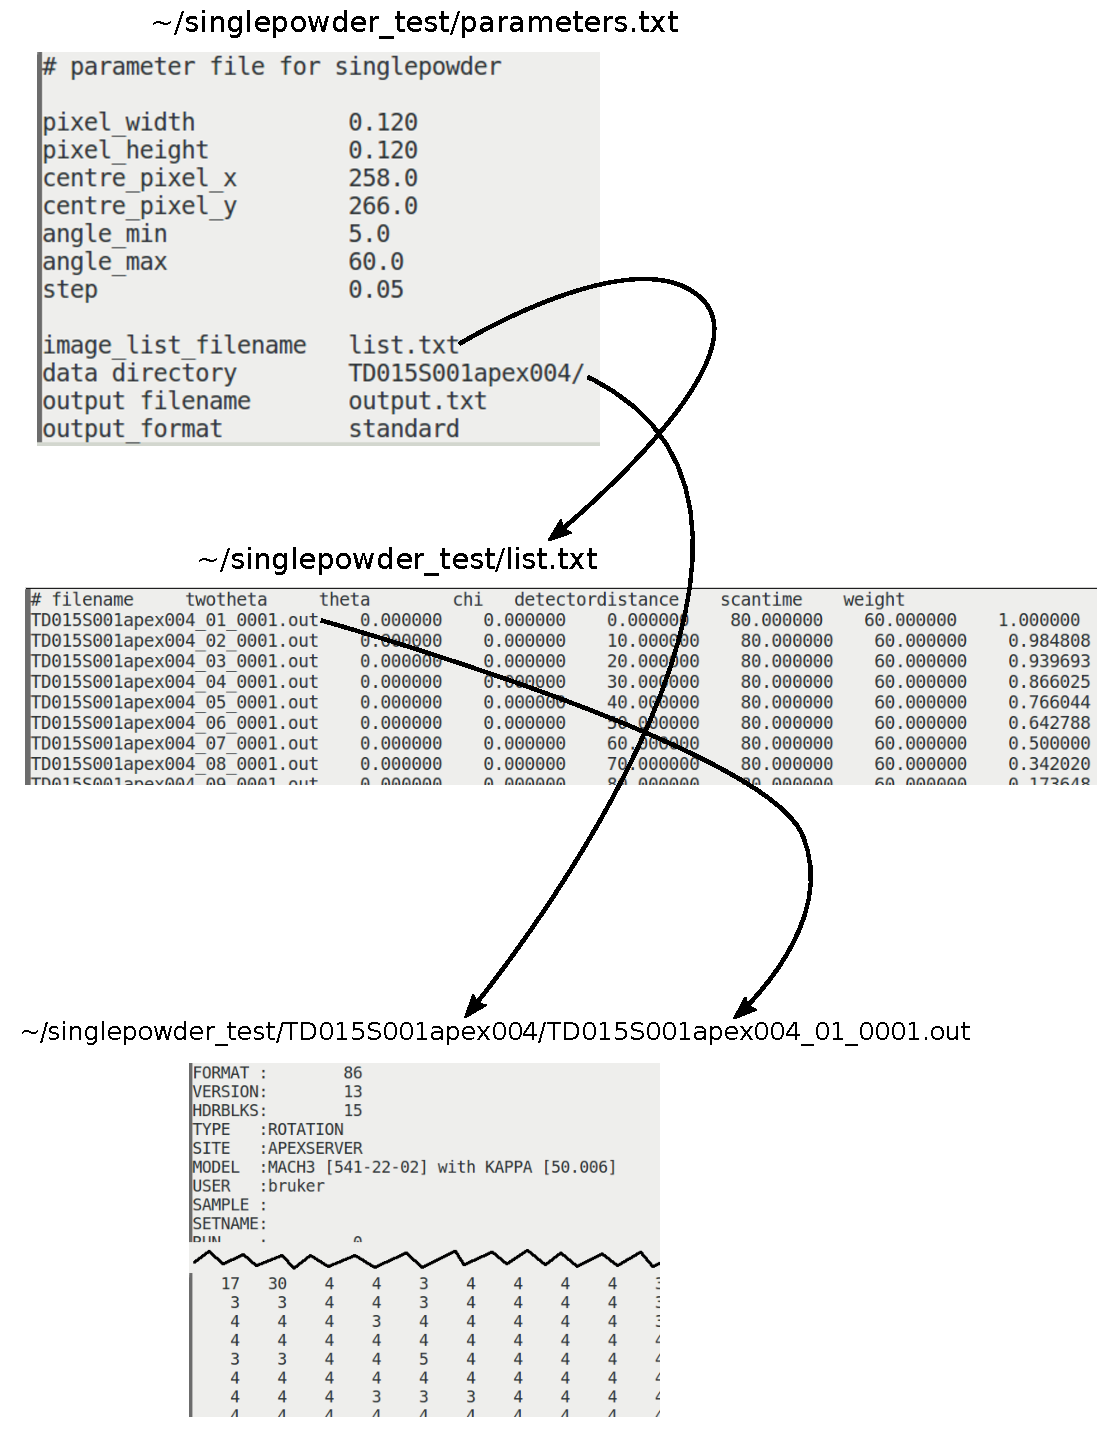
\includegraphics[width=15cm]{figs/files.pdf}
\caption{\label{fig:files}Example for input files. In the directory \texttt{\~{}/singlepowder\_test/}, the command \texttt{singlepowder parameters.txt} runs the program.}
\end{figure}

\subsection{Creating a mask}

The mask is created with the following steps:
\begin{itemize}
\item Averaging many detector images (preferrably without any reflections but just background).
\item Inverting the values.
\item Setting the value for corrupted pixels to zero.
\end{itemize}

Averaging is done using the command

\begin{verbatim}
singlepowder make_mask <data_directory> <list_filename> <output_filename>
\end{verbatim}

Iverting uses the command

\begin{verbatim}
singlepowder invert_mask <old_mask_filename> <new_mask_filename>
\end{verbatim}

For setting currupted pixels to zero, multiply with a mask with 0 for the corrupted pixels and 1 for the others:

\begin{verbatim}
singlepowder multiply_masks <mask_filename1> <mask_filename2> <output_mask_filename>
\end{verbatim}

Example: Assuming, the file \verb|corrupted.txt| contains a mask with corrupted pixels set to 0 and others to 1, the directory \verb|TD015S001apex004| contains the data files and \verb|list.txt| is the list file, the following commands must be executed:

\begin{verbatim}
singlepowder make_mask TD015S001apex004/ list.txt averaged.txt
singlepowder invert_mask averaged.txt inverted.txt
singlepowder multiply_mask corrupted.txt inverted.txt mask.txt
\end{verbatim}

\section{Geometry of the diffractometer}

All lengths are in $ \mathrm{mm} $ and all angles in $ \mathrm{deg} $.

Figure \ref{fig:goniometer} shows a four circle diffractometer. The angles are shown with the directions used in the program (only $ 2\theta $ is actually used so far). In order to avoid confusion, $ 2\theta $ names the position of the detector while "powder angle" $ \varepsilon $ is used for the angle between the diffracted beam and the direct beam for a certain pixel. The pixel indices $ x $ and $ y $ and the pixel width $ w $ and height $ h $ are shown with the direction used by the classes Geometry and DetectorImage.

The variables in the figure and the following calculation refer to the following variables in the program code:

\begin{align*}
	d &: \text{detector\_distance} & (\mathrm{mm})\\
	2\theta &: \text{twotheta} & (\mathrm{deg})\\
	\varepsilon &: \text{powder\_angle} & (\mathrm{deg})\\
	x &: \text{pixel\_x} & (\mathrm{index})\\
	y &: \text{pixel\_y} & (\mathrm{index})\\
	w &: \text{pixel\_width} & (\mathrm{mm})\\
	h &: \text{pixel\_height} & (\mathrm{mm})\\
	x_c &: \text{centre\_pixel\_x} & (\mathrm{index})\\
	y_c &: \text{centre\_pixel\_y} & (\mathrm{index})\\
	\Delta x &: \text{delta\_x} & (\mathrm{mm})\\
	\Delta y &: \text{delta\_y} & (\mathrm{mm})\\
\end{align*}

\begin{figure}
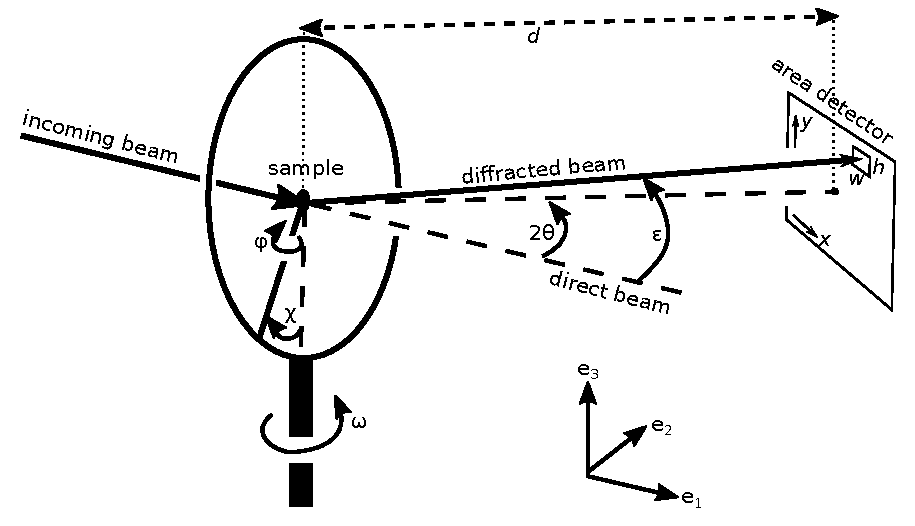
\includegraphics{figs/goniometer.pdf}
\caption{\label{fig:goniometer}Direction of the angles $ 2\theta $, $ \omega $, $ \chi $, $ \varphi $, the pixel indices $ x $, $ y $ and the Cartesian basis vectors $ e_1, e_2, e_3 $.}
\end{figure}

$ x_c $ and $ y_c $ are the indices of the pixel that is hit by the direct beam when all angles are set to zero. The deviation (in mm) from this pixel is for the pixel with indices $ (x, y) $:

\begin{align*}
	\Delta x &= w(x - x_c) \\
	\Delta y &= h(y - y_c) \\
\end{align*}

Using the basis vectors\footnote{The basis vectors are dimensionless and the coordinates have unit $ \mathrm{mm} $.} defined in Figure \ref{fig:goniometer} (the origin is placed at the pivot point of the goniometer, i.e. the sample), we get for $ 2\theta = 0 $ the following coordinates of the pixel:

\begin{align*}
  \boldsymbol{p} = \begin{pmatrix} d \\ -\Delta x \\ \Delta y \end{pmatrix}	
\end{align*}

The rotation matrix around $ e_3 $ depends on $ 2\theta $:

\begin{align*}
	R = \begin{pmatrix}
		    \cos(2\theta) & -\sin(2\theta) & 0 \\
		    \sin(2\theta) & \cos(2\theta)  & 0 \\
		    0 & 0 & 1
		\end{pmatrix}
\end{align*}

The coordinates of the pixel with indices $ (x, y) $ depend on $ d $ and $ 2\theta $ and are thus:

\begin{align*}
	\boldsymbol{p'} &= R \boldsymbol{p} \\
	 &=
	\begin{pmatrix}
	d \cos(2\theta) + \Delta x \sin(2\theta) \\
	d \sin(2\theta) - \Delta x \cos(2\theta) \\
	\Delta y
	\end{pmatrix}
\end{align*}

The direct beam intersects the detector circle in the following point:

\begin{align*}
	\boldsymbol{r} = \begin{pmatrix} d \\ 0 \\ 0 \end{pmatrix}
\end{align*}

For the angle $ \varepsilon $ between the direct and diffracted beam, the following condition holds:

\begin{align*}
	|\boldsymbol{r}| |\boldsymbol{p}| \cos(\varepsilon) = \boldsymbol{r} \cdot \boldsymbol{p'}~~\mathrm{,}
\end{align*}

where $ \cdot $ denotes the scalar product.

From this, we can calculate the powder\_angle $ \varepsilon $ :

\begin{align*}
	\varepsilon &= \arccos \frac{\boldsymbol{r} \cdot \boldsymbol{p'}}{|\boldsymbol{r}||\boldsymbol{p'}|} \\
	&= \arccos \frac{d ( d\cos(2\theta) + \Delta x \sin(2\theta))}{\sqrt{(d\cos(2\theta) + \Delta x \sin(2\theta))^2 + (d\sin(2\theta) - \Delta x \cos(2\theta))^2}~d} \\
	&= \arccos \frac{d\cos(2\theta) + \Delta x \sin(2\theta)}{\sqrt{(d\cos(2\theta) + \Delta x \sin(2\theta))^2 + (d\sin(2\theta) - \Delta x \cos(2\theta))^2}}
\end{align*}

This is the formula in Geometry::calculate\_powderangle().

\section{Integration and error propagation}

The algorithm loops over all pixels of all detector images. For each detector image, the detector distance and $ 2\theta $ are given in the list file. From the geometric parameters, the powder\_angle is calculated. The counts of this pixel are summed in the diffractogram at the according powder\_angle. The bin of the histogram is used, where the angle deviates maximally \verb|step|/2. If the powder\_angle of the pixel lies outside the interval $ [\texttt{angle\_min} - \texttt{step}/2, \texttt{angle\_max} + \texttt{step}/2] $, the counts are discarded. The counts are weighted by the weight given in the list file.

Let $ i, j $ run over all pixels of all detector images for a fixed powder\_angle. The counts are $ c_i $ and the weights $ w_i $. A weight $ w_i $ is the product of the weight of the image (given in the list file) and the weight of the pixel (given in the mask file). The intensity at this angle is:

\begin{align*}
	I &= \frac{\sum\limits_{i = 1}^{n} w_i c_i}{\sum\limits_{j=1}^{n} w_j}
\end{align*}

The error on the counts are $ \sigma_{c_i} = \sqrt{c_i} $, so the error on the intensity can be computed in the following way:

\begin{align*}
	\sigma_I &= \sqrt{\sum\limits_{i=1}^{n} \left(\frac{\partial I}{\partial c_i}\right)^2 \sigma_{c_i}^2} \\
	&= \sqrt{\sum\limits_{i=1}^{n} \left(w_i \middle/ \sum\limits_{j=1}^{n} w_j\right)^2 c_i} \\
	&= \frac{1}{\sum\limits_{j=1}^{n} w_j}~ \sqrt{\sum\limits_{i=1}^{n} w_i^2 c_i}
\end{align*}

During the integration, the following sums are collected for each powder\_angle:

\begin{align*}
	\texttt{sum\_of\_weights} &= \sum\limits_{i=1}^{n} w_i \\
	\texttt{sum\_of\_weighted\_counts} &= \sum\limits_{i=1}^{n} w_i c_i \\
	\texttt{sum\_of\_squareweighted\_counts} &= \sum\limits_{i=1}^{n} w_i^2 c_i
\end{align*}

These values are written to the output file when the parameter \texttt{output\_format} in the parameter file is set to detailed.

The sums are calculated in Diffractogram::add\_counts().

The intensity and its error is then calculated as follows:

\begin{align*}
	\texttt{intensity} &=& I &=& \texttt{sum\_of\_weighted\_counts}\big/\texttt{sum\_of\_weights} \\
	\texttt{error} &=& \sigma_I &=& \sqrt{\texttt{sum\_of\_squareweighted\_counts}}\big/\texttt{sum\_of\_weights}
\end{align*}

This is the formula in Diffractogram::calculate\_intensities\_and\_errors().

\section{Structure of the program}

The structure of the program for integration is shown in Figure \ref{fig:class_diagram}. For the creation of the mask, the class MaskMaker is used.

\begin{figure}
	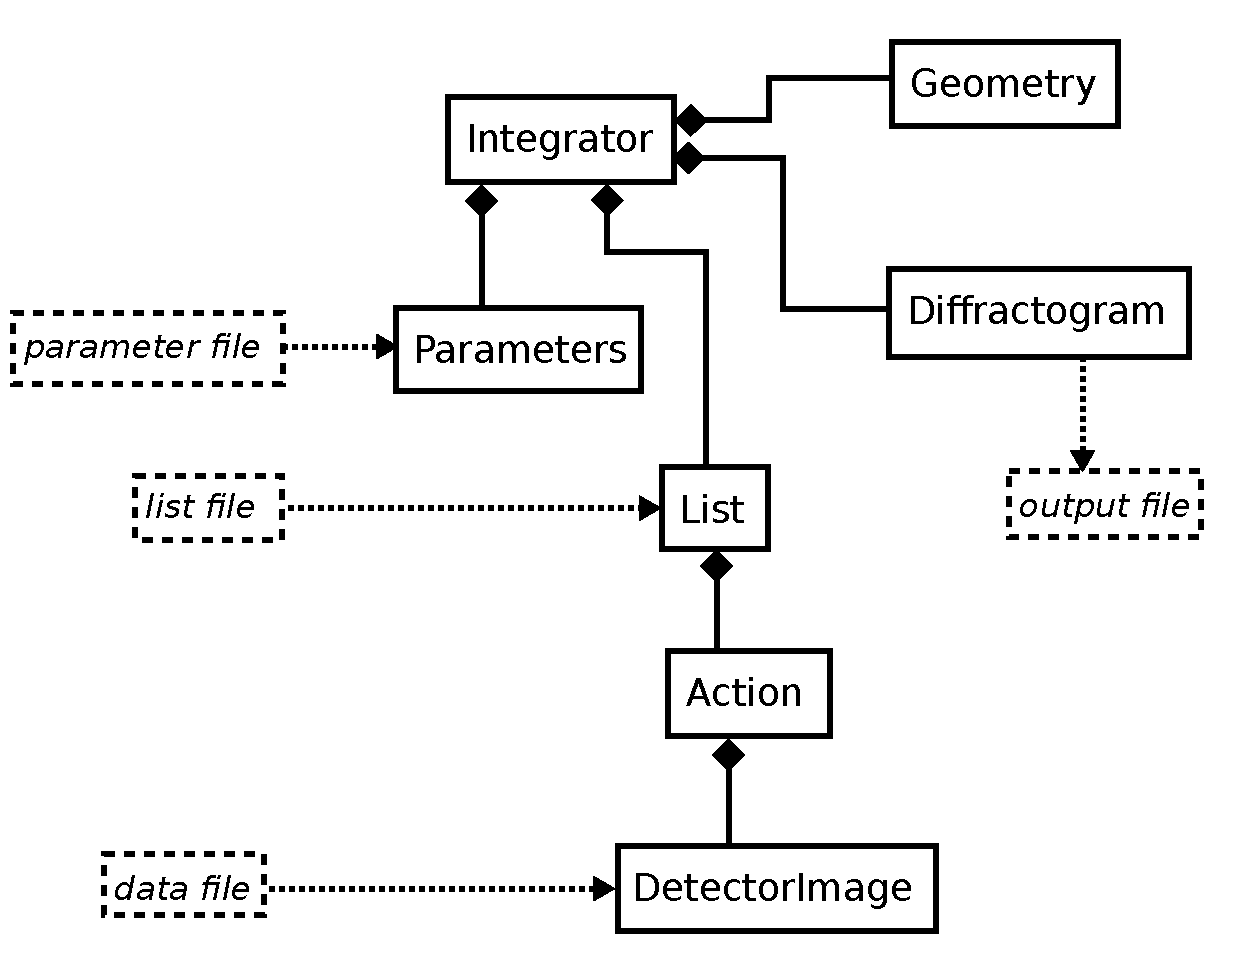
\includegraphics[width=15cm]{figs/class_diagram.pdf}
	\caption{\label{fig:class_diagram}Diagram showing the hierarchy of the classes and the files they read and write.}
\end{figure}

\end{document}